\section{Experimental Results}
\label{sec:experiments}

\subsection{Experimental Setup}


In this milestone report, we show experimental results when we apply KNN method to sequences of CPU usage measurements data.
We used Samsung Galaxy S device on which Android 2.3 Gingerbread is running, and Netflix application was used for collecting CPU usage statistics.
10 movies are selected from \term{Popular on Netflix} section of Netflix website and selected movies are shown in Table \ref{tab:movies}.
CPU statistics of selected movies were captured by recording CPU statistics in 1-second and 5-second intervals using the native UNIX command, \term{top}, while playing the first 30 minutes of each movie. 
The measurement was repeated 5 times for each movie.
Measurement results of two selected movies are previously shown in Figure \ref{fig:preliminaries}.

\begin{table}[h!]
\begin{center}
\begin{tabular}{|c|l|c|l|}
\hline
ID & Movie Title & ID & Movie Title \\ 
\hline
1 & Transformers: Dark of the Moon 		& 6 & Super 8\\
2 & Thor								& 7 & Mean Girls 2 \\
3 & Hachi: A Dog's Tale 					& 8 & Captain America \\
4 & The True Story of Puss 'n Boots 		& 9 &  Snatch \\
5 & Wallace \& Gromit: Loaf and Death 		& 10 & No Strings Attached \\
\hline
\end{tabular}
\end{center}
\caption{Selected Movies}
\label{tab:movies}
\end{table}

\subsection{Fast Subsequence Matching Algorithm Results}
Query subsequences are chosen from a 30-min length sequence with varying starting index and length. At every 60 sec, the subsequence was extracted with length, $l = (180, 240, 300, 600, 900, 1200)$. 

\subsection{KNN Experiment Results}

For each movie, one of five CPU usage sequence is selected as test data and the rest four sequences are considered as training data set. 
The length of subsequence varying from 60 seconds to 360 seconds is set and each test and training data is divided based on the subsequence length as described in \ref{sec:knn}.
When dividing sequence data, we adopt a concept of sliding window which moves by 1 step size.
Each data sequence consists of $360$ measurement points, and therefore $(360 - subsequence\_length + 1)$ subsequences are generated from the data sequence. 

After building up test data set and training data set by generating subsequences, we apply KNN method in order to classify each subsequence of test data based on training data set. 
In this experiment, $k$ value is set to 3 for the simplicity.
The accuracy of classification according to the length of subsequence is shown in Figure \ref{fig:experiment_knn}.
The accuracy is low as 46$\%$ when subsequence length is set to 60-second.
However, the accuracy increases up to 88$\%$ when subsequence is set to 180-second.
The experimental result shows that given 10 movies and CPU usage statistics of 150 seconds, our side channel attack correctly predicts which movie a user is watching at the accuracy of higher than 80$\%$.

\begin{figure}[!h]
\centering
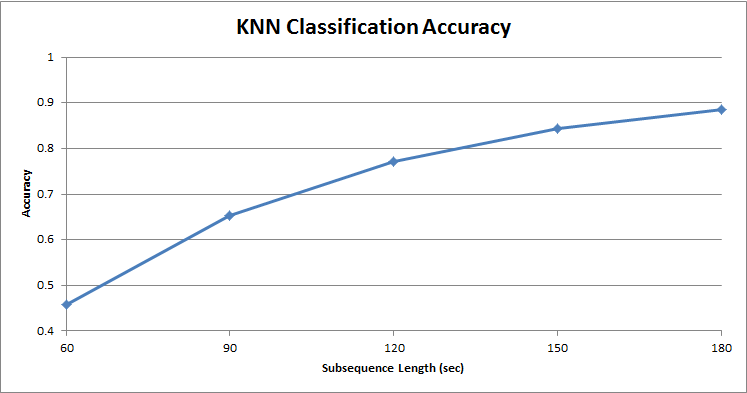
\includegraphics[scale=0.50]{Figures/experiment_knn}
\caption{KNN Classification Accuracy}
\label{fig:experiment_knn}
\vspace{-5mm}
\end{figure}